\begin{figure}
	\centering
	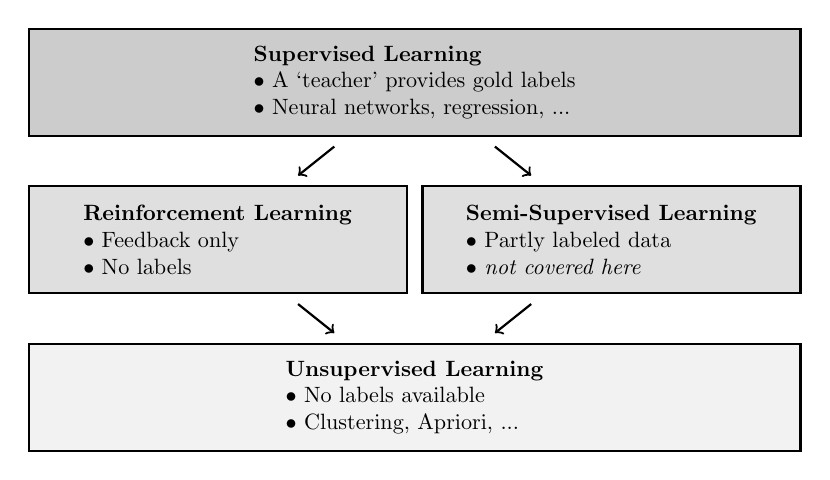
\begin{tikzpicture}[
		scale=0.5,
		every node/.style={scale=0.8},
		block/.style={
			draw=black,
			thick,
			align=left,
			minimum height=17mm,
			minimum width=60mm
		},
		arrow/.style={
			shorten >=0.2cm,
			shorten <=0.2cm,
			->,
			thick
		}
	]
	
		\node[block,minimum width=122.5mm,fill=lightgray!80] (A) at (0,4) {
			\textbf{Supervised Learning} \\
			$\bullet$ A `teacher' provides gold labels \\
			$\bullet$ Neural networks, regression, ...
		};

		\node[block,fill=lightgray!50] (B) at (-5,0) {
			\textbf{Reinforcement Learning} \\
			$\bullet$ Feedback only \\
			$\bullet$ No labels
		};

		\node[block,fill=lightgray!50] (C) at (5,0) {
			\textbf{Semi-Supervised Learning} \\
			$\bullet$ Partly labeled data \\
			$\bullet$ \textit{not covered here}
		};

		\node[block,minimum width=122.5mm,fill=lightgray!20] (D) at (0,-4) {
			\textbf{Unsupervised Learning} \\
			$\bullet$ No labels available \\
			$\bullet$ Clustering, Apriori, ...
		};
	
		\draw[arrow] (A) -- (B);
		\draw[arrow] (A) -- (C);
		\draw[arrow] (B) -- (D);
		\draw[arrow] (C) -- (D);

	\end{tikzpicture}
\end{figure}